\documentclass[12pt]{article}

\usepackage[a4paper,margin=1in]{geometry}
\usepackage{amsmath,amssymb}
\usepackage{newtxtext,newtxmath} % Times-style font
\usepackage{fancyhdr}
\usepackage{listings}
\usepackage{graphicx}
\usepackage{float}
\usepackage{algorithm}
\usepackage{algpseudocode}
\usepackage{booktabs}
\usepackage{xcolor}

\setlength{\textfloatsep}{10pt}
\setlength{\floatsep}{10pt}

\setlength{\parindent}{0pt}
\setlength{\parskip}{5pt}

% Keep entire document at 12 pt
\AtBeginDocument{
    \fontsize{12pt}{14pt}\selectfont
}

\lstdefinestyle{code}{
    language=Python,
    basicstyle=\ttfamily\fontsize{10pt}{12pt}\selectfont,
    breaklines=true,
    breakatwhitespace=false,
    frame=single,
    numbers=left,
    numberstyle=\tiny\color{gray},
    keywordstyle=\color{blue},
    commentstyle=\color{gray},
    stringstyle=\color{green!50!black},
    columns=fullflexible,
    keepspaces=true,
    showstringspaces=false
}

\lstdefinestyle{output}{
    basicstyle=\ttfamily\fontsize{9.5pt}{11.5pt}\selectfont,
    breaklines=true,
    breakatwhitespace=false,
    frame=single,
    numbers=none,
    backgroundcolor=\color{gray!6},
    columns=fullflexible,
    keepspaces=true,
    showstringspaces=false
}

% ------------------------------------------------
% Header
% ------------------------------------------------

\pagestyle{fancy}
\fancyhf{}

\fancyhead[L]{Name: Kishan Sahu{\hspace{4cm}}}
\fancyhead[R]{Enrollment No.: P26DS017{\hspace{3.5cm}}}

\renewcommand{\headrulewidth}{0.4pt}
\setlength{\headheight}{15pt}

% ------------------------------------------------
% Code formatting
% ------------------------------------------------

\lstset{
    basicstyle=\ttfamily\fontsize{10pt}{12pt}\selectfont,
    breaklines=true,
    frame=single,
    columns=fullflexible,
    keepspaces=true,
    showstringspaces=false
}

\begin{document}

% ------------------------------------------------
% TITLE
% ------------------------------------------------

\begin{center}
\textbf{Computer Science and Engineering Department, SVNIT, Surat}\\
\textbf{M.Tech. I -- Semester I}\\
\textbf{Machine Learning (CSDS105)}\\
\textbf{Lab Assignment 3: Classification using Decision Tree and K-Nearest Neighbors}
\end{center}

\vspace{0.3cm}

\section{Introduction and Problem Formulation}

Supervised machine learning algorithms for classification aim to map input feature vectors $\mathbf{x} \in \mathbb{R}^d$ to categorical class labels $y \in \mathcal{C}$. This experimental study benchmarks and contrasts two classical classification paradigms:
\begin{enumerate}
    \item \textbf{Decision Tree Classifier}: A non-parametric, eager learning model that partitions the feature space recursively into axis-aligned rectangular regions using information-theoretic criteria.
    \item \textbf{K-Nearest Neighbors (KNN) Classifier}: An instance-based, non-parametric lazy learner that estimates local posterior class probabilities based on spatial proximity metrics.
\end{enumerate}

\subsection{Dataset Selection: Breast Cancer Wisconsin Diagnostic}
To rigorously evaluate both models, the \textbf{Breast Cancer Wisconsin (Diagnostic)} dataset is selected from \texttt{sklearn.datasets}. 
\begin{itemize}
    \item \textbf{Sample Size}: 569 instances (212 Malignant, 357 Benign).
    \item \textbf{Feature Dimensionality}: 30 continuous real-valued features computed from digitized images of fine needle aspirate (FNA) of breast masses (e.g., radius, texture, perimeter, area, smoothness, compactness, concavity).
    \item \textbf{Suitability for Decision Tree}: The high feature count with non-linear relationships enables multi-stage feature selection and threshold partitioning without trivial 1-feature shortcuts.
    \item \textbf{Suitability for KNN}: Continuous metric space with heterogeneous feature scales illustrates the absolute necessity of standard scaling ($z$-score normalization) for isotropic distance computation.
\end{itemize}

\section{Environment Setup and Data Preprocessing}

\subsection{Environment Setup}
The implementation utilizes standard scientific Python libraries: NumPy for array computation, Pandas for tabular data management, Matplotlib and Seaborn for plotting, and Scikit-Learn for machine learning estimators and metrics.

\begin{lstlisting}[style=code]
import numpy as np
import pandas as pd
import matplotlib.pyplot as plt
import seaborn as sns

from sklearn.datasets import load_breast_cancer
from sklearn.model_selection import train_test_split
from sklearn.preprocessing import StandardScaler
from sklearn.tree import DecisionTreeClassifier, plot_tree
from sklearn.neighbors import KNeighborsClassifier
from sklearn.metrics import (
    confusion_matrix,
    ConfusionMatrixDisplay,
    classification_report,
    accuracy_score,
    precision_score,
    recall_score,
    f1_score,
    zero_one_loss
)

# Set consistent plotting aesthetics
plt.style.use('seaborn-v0_8-whitegrid' if 'seaborn-v0_8-whitegrid' in plt.style.available else 'default')
plt.rcParams['font.sans-serif'] = 'DejaVu Sans'
plt.rcParams['figure.dpi'] = 120
plt.rcParams['axes.titlesize'] = 14
plt.rcParams['axes.labelsize'] = 12

print("Dependencies successfully imported.")
\end{lstlisting}

\begin{lstlisting}[style=output]
Dependencies successfully imported.
\end{lstlisting}

\subsection{Dataset Ingestion}
The dataset is loaded directly into feature matrix $\mathbf{X}$ and target vector $\mathbf{y}$. Class distribution is inspected to verify stratification requirements.

\begin{lstlisting}[style=code]
# Load the raw dataset
cancer = load_breast_cancer()
X = pd.DataFrame(cancer.data, columns=cancer.feature_names)
y = pd.Series(cancer.target, name='diagnosis')
target_names = cancer.target_names  # ['malignant', 'benign']

print(f"Dataset Shape: {X.shape[0]} samples, {X.shape[1]} features")
print(f"Target Classes: {dict(enumerate(target_names))}")
print(f"Class Distribution:\n{y.value_counts(normalize=True).rename(index=dict(enumerate(target_names))) * 100}\n")
X.head(3)
\end{lstlisting}

\begin{lstlisting}[style=output]
Dataset Shape: 569 samples, 30 features
Target Classes: {0: 'malignant', 1: 'benign'}
Class Distribution:
diagnosis
benign       62.741652
malignant    37.258348
Name: proportion, dtype: float64
\end{lstlisting}

\subsection{Stratified Train-Test Split and Standardization}
A stratified 75/25 split is executed with seed $42$. For distance-sensitive KNN modeling, standard scaling is fit strictly on the training partition and transformed across both sets:
\begin{equation}
    z_{ij} = \frac{x_{ij} - \mu_j}{\sigma_j}
\end{equation}
where $\mu_j$ is the empirical feature mean and $\sigma_j$ is the standard deviation. Unscaled features are retained for the Decision Tree to demonstrate scale invariance.

\begin{lstlisting}[style=code]
# Perform Stratified Train-Test Split
X_train, X_test, y_train, y_test = train_test_split(
    X, y,
    test_size=0.25,
    random_state=42,
    stratify=y
)

print(f"Training set: {X_train.shape[0]} samples")
print(f"Testing set:  {X_test.shape[0]} samples")

# Feature Scaling: Essential for distance-based algorithms (KNN)
scaler = StandardScaler()
X_train_scaled = scaler.fit_transform(X_train)
X_test_scaled = scaler.transform(X_test)

# Convert back to DataFrame for clean indexing
X_train_scaled = pd.DataFrame(X_train_scaled, columns=X.columns)
X_test_scaled = pd.DataFrame(X_test_scaled, columns=X.columns)

print("Scaling complete: Mean ~ 0, Variance ~ 1 on training set.")
\end{lstlisting}

\begin{lstlisting}[style=output]
Training set: 426 samples
Testing set:  143 samples
Scaling complete: Mean ~ 0, Variance ~ 1 on training set.
\end{lstlisting}

\newpage
\section{Decision Tree Classifier}

\subsection{Mathematical Formulations of Node Splitting}
At each node, the decision tree selects an optimal feature $A$ and splitting threshold $\theta$ that maximizes the reduction in node impurity.

\subsubsection{1. Entropy}
Entropy quantifies the uncertainty or impurity of a sample subset $S$ comprising $c$ discrete classes:
\begin{equation}
    H(S) = - \sum_{i=1}^{c} p_i \log_2(p_i)
\end{equation}
where $p_i = \frac{|S_i|}{|S|}$ denotes the relative proportion of samples belonging to class $i$. For binary diagnostic classification ($c=2$):
\begin{equation}
    H(S) = - p_0 \log_2(p_0) - p_1 \log_2(p_1)
\end{equation}
\begin{itemize}
    \item If all samples belong to one class (completely pure), $H(S) = 0$.
    \item If classes are uniformly distributed ($p_0 = p_1 = 0.5$), $H(S) = 1.0$ (maximum impurity).
\end{itemize}

\subsubsection{2. Information Gain ($IG$)}
Information Gain measures the expected reduction in entropy attained by partitioning subset $S$ along attribute $A$ into partitions $\{S_v\}$:
\begin{equation}
    IG(S, A) = H(S) - \sum_{v \in \text{Values}(A)} \frac{|S_v|}{|S|} H(S_v)
\end{equation}
The optimal split $(A^*, \theta^*)$ chosen at each node satisfies:
\begin{equation}
    (A^*, \theta^*) = \arg\max_{A, \theta} IG(S, A, \theta)
\end{equation}

\subsubsection{3. Alternative Impurity Metric: Gini Impurity}
The Gini Index represents the expected error rate if a randomly drawn element is labeled randomly according to the class distribution:
\begin{equation}
    \text{Gini}(S) = 1 - \sum_{i=1}^{c} p_i^2
\end{equation}
For a binary evenly distributed split, $\text{Gini}(S) = 1 - (0.5^2 + 0.5^2) = 0.5$.

\subsection{Decision Tree Training and Visualization}
A Decision Tree with entropy criterion and maximum depth 4 is trained on the training partition. Restricting depth prevents excessive branch clutter and ensures the structural tree logic is fully interpretable.

\begin{lstlisting}[style=code]
# Train Decision Tree with Entropy criterion
dt_model = DecisionTreeClassifier(criterion='entropy', max_depth=4, random_state=42)
dt_model.fit(X_train, y_train)

# Visualize the Decision Tree
fig, ax = plt.subplots(figsize=(18, 10))
plot_tree(
    dt_model,
    feature_names=cancer.feature_names,
    class_names=target_names,
    filled=True,
    rounded=True,
    fontsize=10,
    ax=ax
)
plt.title("Decision Tree Structure (Criterion: Entropy, Max Depth: 4)", fontsize=16, fontweight='bold', pad=15)
plt.tight_layout()
plt.show()
\end{lstlisting}

\begin{figure}[H]
    \centering
    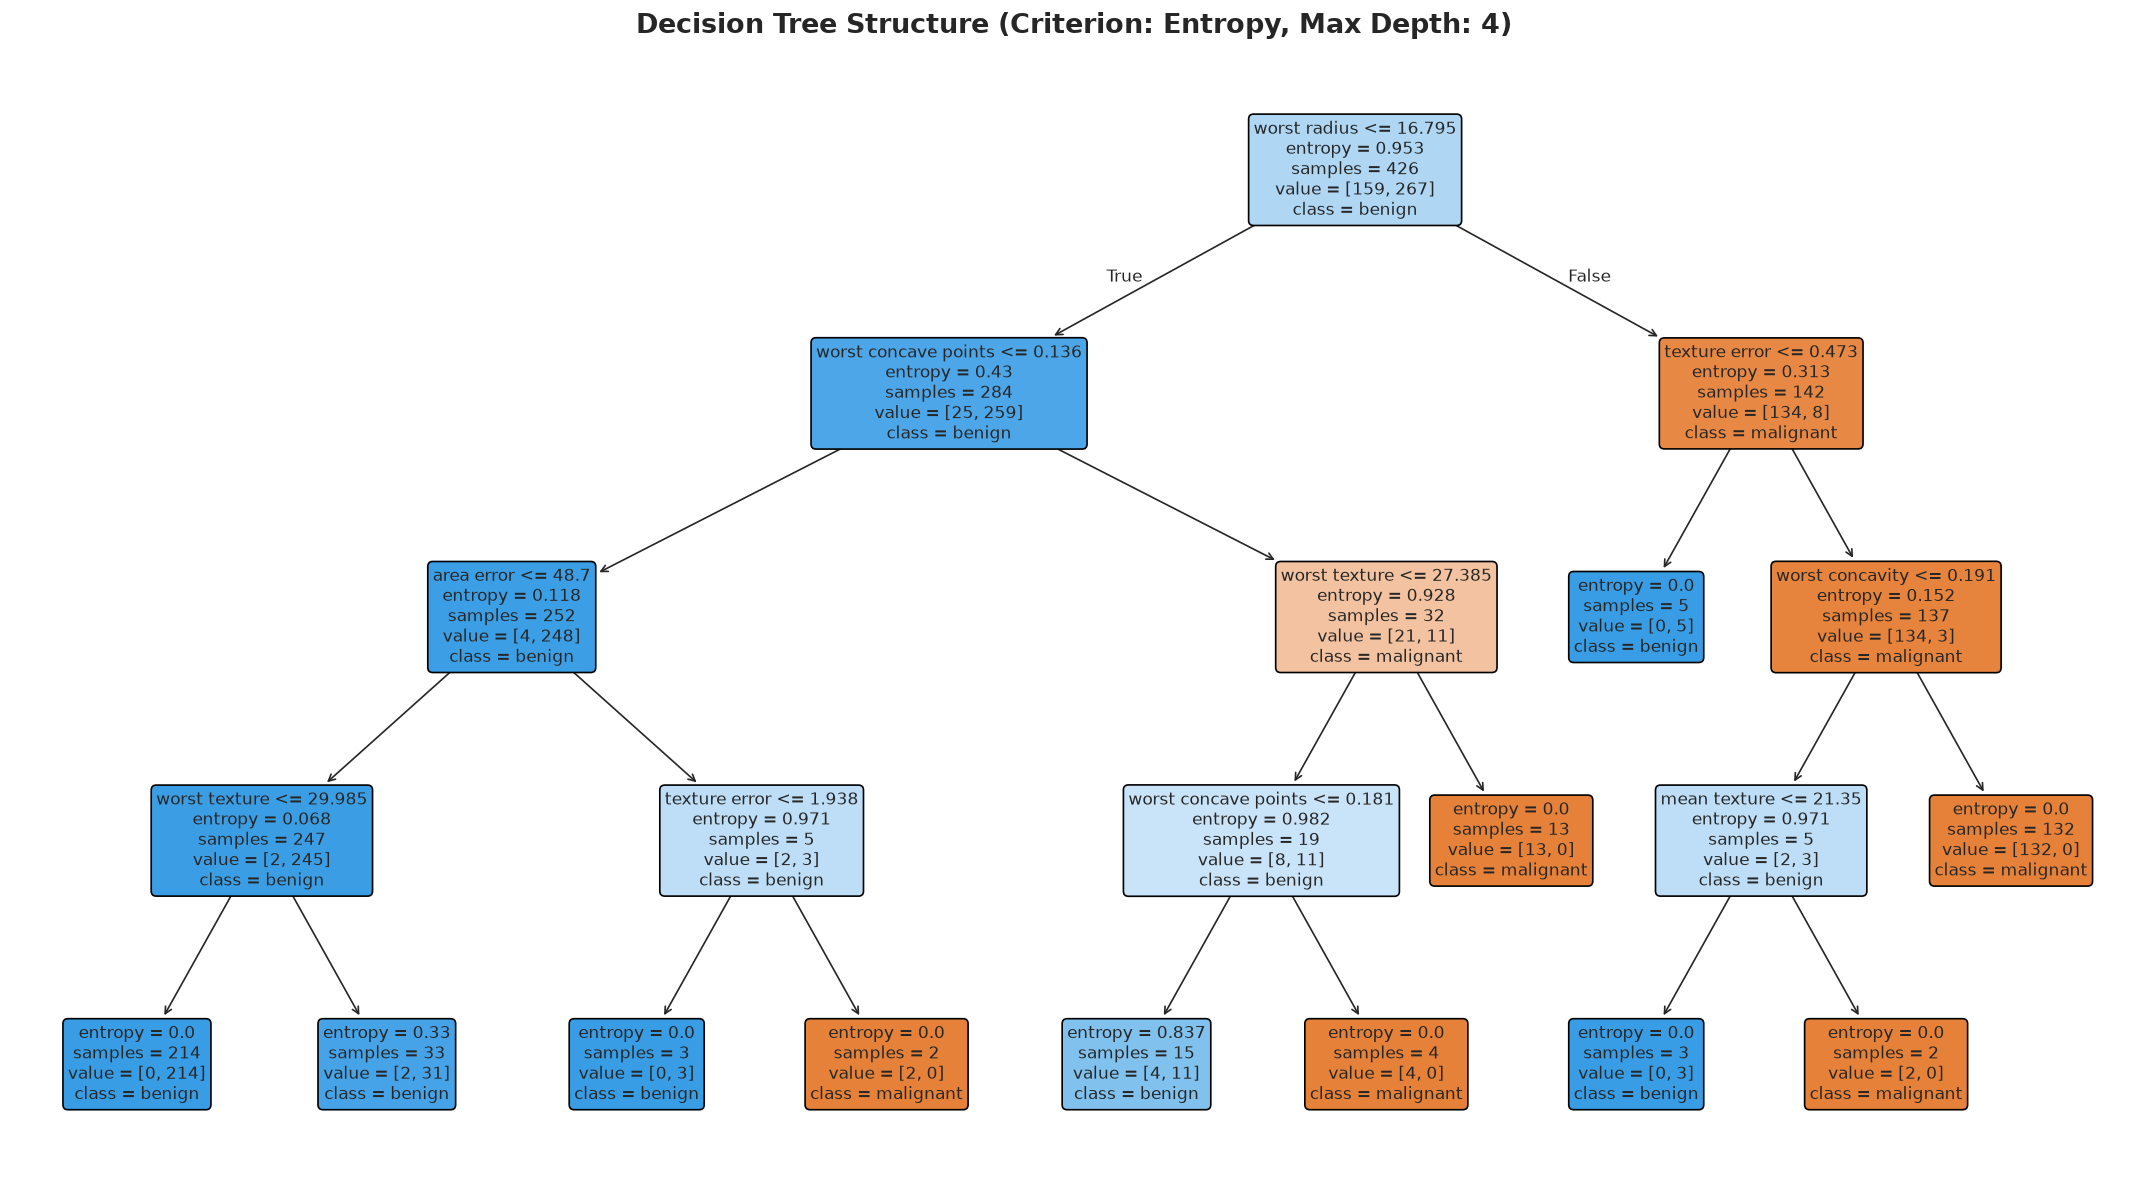
\includegraphics[width=0.98\textwidth]{figures/dt_tree_structure.png}
    \caption{Visualized Decision Tree hierarchy showing internal decision nodes, splitting thresholds, sample counts, entropy values, and dominant class colorings.}
    \label{fig:dt_tree}
\end{figure}

\subsection{Decision Tree Evaluation and Confusion Matrix}
Predictions on the unseen testing set $\mathbf{X}_{\text{test}}$ are evaluated using the Confusion Matrix and associated diagnostic metrics:
\begin{align}
    \text{Accuracy} &= \frac{TP + TN}{TP + TN + FP + FN} \\
    \text{Precision} &= \frac{TP}{TP + FP} \\
    \text{Recall} &= \frac{TP}{TP + FN} \\
    \text{F1-Score} &= 2 \times \frac{\text{Precision} \times \text{Recall}}{\text{Precision} + \text{Recall}} \\
    \text{Misclassification Error} &= 1 - \text{Accuracy} = \frac{FP + FN}{N}
\end{align}

\begin{lstlisting}[style=code]
y_pred_dt = dt_model.predict(X_test)

# Calculate metrics
dt_acc = accuracy_score(y_test, y_pred_dt)
dt_prec = precision_score(y_test, y_pred_dt)
dt_rec = recall_score(y_test, y_pred_dt)
dt_f1 = f1_score(y_test, y_pred_dt)
dt_error = zero_one_loss(y_test, y_pred_dt)

# Plot Confusion Matrix
cm_dt = confusion_matrix(y_test, y_pred_dt)
fig, ax = plt.subplots(figsize=(6, 5))
sns.heatmap(
    cm_dt,
    annot=True,
    fmt='d',
    cmap='Blues',
    xticklabels=target_names,
    yticklabels=target_names,
    cbar=False,
    ax=ax
)
ax.set_title("Decision Tree: Confusion Matrix", fontweight='bold')
ax.set_xlabel("Predicted Label")
ax.set_ylabel("True Label")
plt.tight_layout()
plt.show()

print(f"=== Decision Tree Evaluation Metrics ===")
print(f"Accuracy:                 {dt_acc:.4f} ({dt_acc*100:.2f}%)")
print(f"Precision (Benign):       {dt_prec:.4f}")
print(f"Recall (Benign):          {dt_rec:.4f}")
print(f"F1-Score:                 {dt_f1:.4f}")
print(f"Misclassification Error:  {dt_error:.4f} ({dt_error*100:.2f}%)\n")
print("Detailed Classification Report:")
print(classification_report(y_test, y_pred_dt, target_names=target_names))
\end{lstlisting}

\begin{figure}[H]
    \centering
    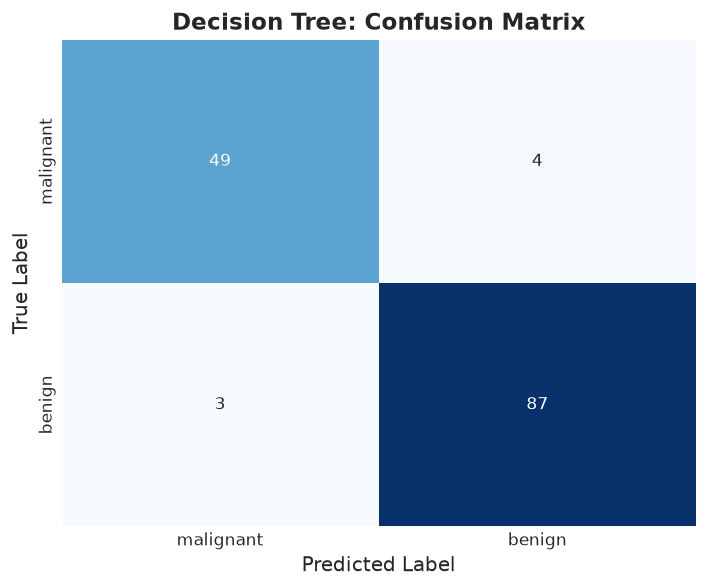
\includegraphics[width=0.48\textwidth]{figures/dt_confusion_matrix.png}
    \caption{Decision Tree Confusion Matrix on test samples ($N=143$).}
    \label{fig:dt_cm}
\end{figure}

\begin{lstlisting}[style=output]
=== Decision Tree Evaluation Metrics ===
Accuracy:                 0.9510 (95.10%)
Precision (Benign):       0.9560
Recall (Benign):          0.9667
F1-Score:                 0.9613
Misclassification Error:  0.0490 (4.90%)

Detailed Classification Report:
              precision    recall  f1-score   support

   malignant       0.94      0.92      0.93        53
      benign       0.96      0.97      0.96        90

    accuracy                           0.95       143
   macro avg       0.95      0.95      0.95       143
weighted avg       0.95      0.95      0.95       143
\end{lstlisting}

\subsection{Decision Tree Parametric Error Curve: Error vs. Max Depth}
To examine model bias-variance trade-offs, misclassification error rates are evaluated on both training and testing partitions for $\text{max\_depth} \in [1, 15]$.

\begin{lstlisting}[style=code]
depths = list(range(1, 16))
dt_train_errors = []
dt_test_errors = []

for depth in depths:
    clf = DecisionTreeClassifier(criterion='entropy', max_depth=depth, random_state=42)
    clf.fit(X_train, y_train)
    
    train_err = 1.0 - accuracy_score(y_train, clf.predict(X_train))
    test_err = 1.0 - accuracy_score(y_test, clf.predict(X_test))
    
    dt_train_errors.append(train_err)
    dt_test_errors.append(test_err)

best_depth = depths[np.argmin(dt_test_errors)]
min_dt_error = min(dt_test_errors)

plt.figure(figsize=(9, 5))
plt.plot(depths, dt_train_errors, marker='o', label='Training Error Rate', color='#2b5c8f', linewidth=2)
plt.plot(depths, dt_test_errors, marker='s', label='Testing Error Rate', color='#d95f02', linewidth=2)
plt.axvline(x=best_depth, color='green', linestyle='--', label=f'Optimal Depth = {best_depth} (Error = {min_dt_error:.3f})')

plt.title("Decision Tree: Error Rate vs. Tree Max Depth", fontweight='bold')
plt.xlabel(r"Max Depth ($max\_depth$)")
plt.ylabel("Misclassification Error Rate ($1 - Accuracy$)")
plt.xticks(depths)
plt.legend(frameon=True)
plt.tight_layout()
plt.show()

print(f"Optimal Decision Tree Max Depth: {best_depth} with Test Error: {min_dt_error:.4f} (Accuracy: {1-min_dt_error:.4f})")
\end{lstlisting}

\begin{figure}[H]
    \centering
    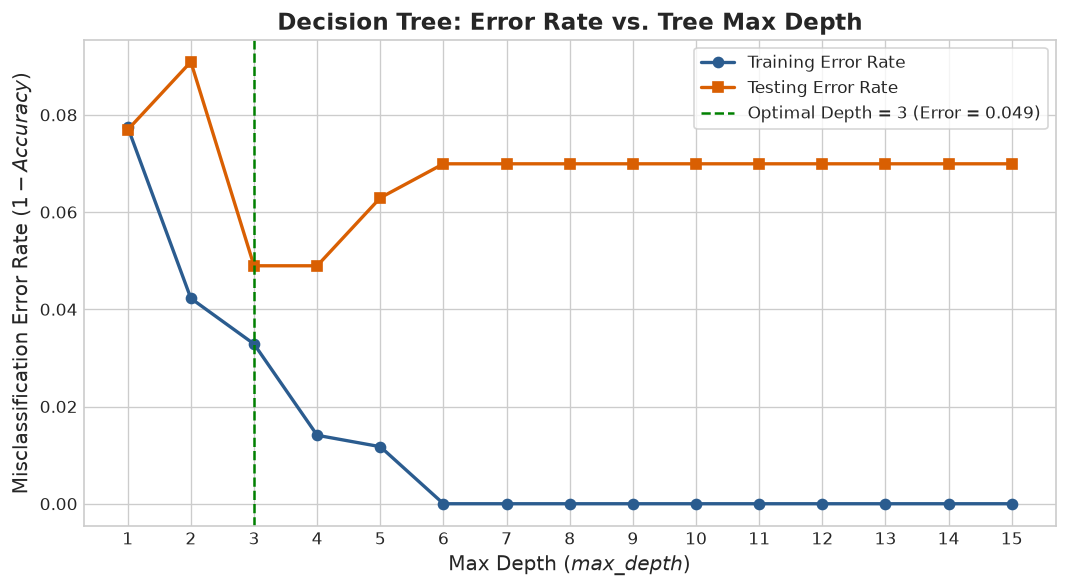
\includegraphics[width=0.72\textwidth]{figures/dt_error_vs_depth.png}
    \caption{Decision Tree Error Rate vs. Maximum Tree Depth showing training error convergence to 0 and optimal test generalization at depth 3.}
    \label{fig:dt_depth_curve}
\end{figure}

\begin{lstlisting}[style=output]
Optimal Decision Tree Max Depth: 3 with Test Error: 0.0490 (Accuracy: 0.9510)
\end{lstlisting}

\newpage
\section{K-Nearest Neighbors (KNN) Classifier}

\subsection{Mathematical Formulations of Distance Metrics}
K-Nearest Neighbors predicts query point labels by computing distance across all training exemplars and applying majority voting among the closest $K$ neighbors.

\subsubsection{1. Euclidean Distance ($L_2$ Norm)}
The geometric straight-line metric in $\mathbb{R}^n$:
\begin{equation}
    d_{\text{Euclidean}}(\mathbf{p}, \mathbf{q}) = \sqrt{\sum_{i=1}^{n} (p_i - q_i)^2} = \|\mathbf{p} - \mathbf{q}\|_2
\end{equation}

\subsubsection{2. Manhattan Distance ($L_1$ Norm)}
The grid/taxicab metric summing coordinate-wise absolute deviations:
\begin{equation}
    d_{\text{Manhattan}}(\mathbf{p}, \mathbf{q}) = \sum_{i=1}^{n} |p_i - q_i| = \|\mathbf{p} - \mathbf{q}\|_1
\end{equation}

\subsubsection{3. Minkowski Distance ($L_p$ Metric Generalization)}
The unified $L_p$ metric parameterized by order $p \ge 1$:
\begin{equation}
    d_{\text{Minkowski}}(\mathbf{p}, \mathbf{q}) = \left( \sum_{i=1}^{n} |p_i - q_i|^p \right)^{\frac{1}{p}}
\end{equation}
When $p=1$, it reduces to Manhattan distance; when $p=2$, it corresponds to Euclidean distance.

\subsubsection{4. Majority Voting Rule}
Given neighborhood set $N_K(\mathbf{x})$ comprising the $K$ closest instances to query point $\mathbf{x}$, the predicted label $\hat{y}$ is:
\begin{equation}
    \hat{y} = \arg\max_{c \in \mathcal{C}} \sum_{i \in N_K(\mathbf{x})} I(y^{(i)} = c)
\end{equation}
where $I(\cdot)$ is the indicator function ($1$ if argument is true, $0$ otherwise).

\subsection{KNN Training and Confusion Matrix}
The KNN estimator is initialized with $K=5$ and trained on standardized feature matrix $\mathbf{X}_{\text{train\_scaled}}$.

\begin{lstlisting}[style=code]
# Train initial KNN model with K=5
knn_model = KNeighborsClassifier(n_neighbors=5, metric='minkowski', p=2)
knn_model.fit(X_train_scaled, y_train)

y_pred_knn = knn_model.predict(X_test_scaled)

# Calculate metrics
knn_acc = accuracy_score(y_test, y_pred_knn)
knn_prec = precision_score(y_test, y_pred_knn)
knn_rec = recall_score(y_test, y_pred_knn)
knn_f1 = f1_score(y_test, y_pred_knn)
knn_error = zero_one_loss(y_test, y_pred_knn)

# Plot Confusion Matrix
cm_knn = confusion_matrix(y_test, y_pred_knn)
fig, ax = plt.subplots(figsize=(6, 5))
sns.heatmap(
    cm_knn,
    annot=True,
    fmt='d',
    cmap='Greens',
    xticklabels=target_names,
    yticklabels=target_names,
    cbar=False,
    ax=ax
)
ax.set_title("KNN (K=5): Confusion Matrix", fontweight='bold')
ax.set_xlabel("Predicted Label")
ax.set_ylabel("True Label")
plt.tight_layout()
plt.show()

print(f"=== KNN (K=5) Evaluation Metrics ===")
print(f"Accuracy:                 {knn_acc:.4f} ({knn_acc*100:.2f}%)")
print(f"Precision (Benign):       {knn_prec:.4f}")
print(f"Recall (Benign):          {knn_rec:.4f}")
print(f"F1-Score:                 {knn_f1:.4f}")
print(f"Misclassification Error:  {knn_error:.4f} ({knn_error*100:.2f}%)\n")
print("Detailed Classification Report:")
print(classification_report(y_test, y_pred_knn, target_names=target_names))
\end{lstlisting}

\begin{figure}[H]
    \centering
    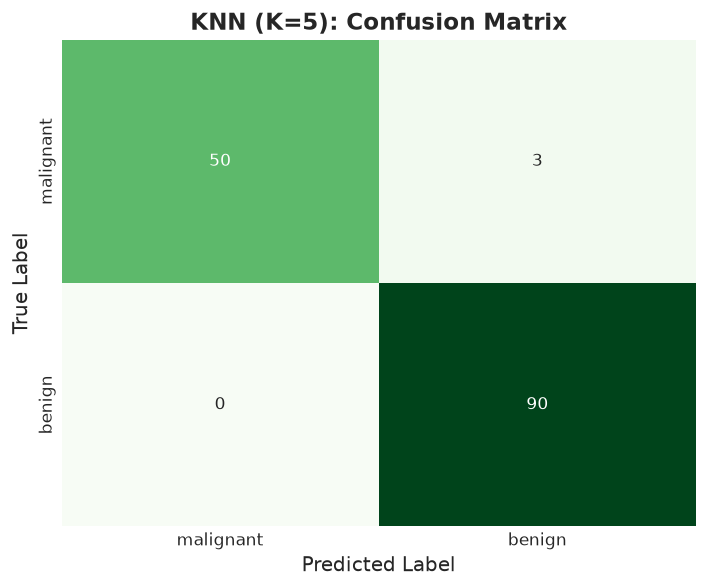
\includegraphics[width=0.48\textwidth]{figures/knn_confusion_matrix.png}
    \caption{KNN ($K=5$) Confusion Matrix on standardized test samples ($N=143$).}
    \label{fig:knn_cm}
\end{figure}

\begin{lstlisting}[style=output]
=== KNN (K=5) Evaluation Metrics ===
Accuracy:                 0.9790 (97.90%)
Precision (Benign):       0.9677
Recall (Benign):          1.0000
F1-Score:                 0.9836
Misclassification Error:  0.0210 (2.10%)

Detailed Classification Report:
              precision    recall  f1-score   support

   malignant       1.00      0.94      0.97        53
      benign       0.97      1.00      0.98        90

    accuracy                           0.98       143
   macro avg       0.98      0.97      0.98       143
weighted avg       0.98      0.98      0.98       143
\end{lstlisting}

\subsection{KNN Parametric Error Curve: Error Rate vs. Neighbor Count ($K$)}
The value of $K$ dictates the bias-variance trade-off:
\begin{itemize}
    \item When $K=1$, the estimator memorizes training observations ($\text{Train Error} = 0$), yielding high variance and noise sensitivity.
    \item As $K$ grows excessively large, local decision boundaries blur into the global class prior, increasing bias.
\end{itemize}
The error rate is empirically tracked across $K \in [1, 30]$.

\begin{lstlisting}[style=code]
k_range = list(range(1, 31))
knn_train_errors = []
knn_test_errors = []

for k in k_range:
    knn = KNeighborsClassifier(n_neighbors=k, metric='minkowski', p=2)
    knn.fit(X_train_scaled, y_train)
    
    train_err = 1.0 - accuracy_score(y_train, knn.predict(X_train_scaled))
    test_err = 1.0 - accuracy_score(y_test, knn.predict(X_test_scaled))
    
    knn_train_errors.append(train_err)
    knn_test_errors.append(test_err)

best_k = k_range[np.argmin(knn_test_errors)]
min_knn_error = min(knn_test_errors)

plt.figure(figsize=(10, 5))
plt.plot(k_range, knn_train_errors, marker='o', label='Training Error Rate', color='#2b5c8f', linewidth=2)
plt.plot(k_range, knn_test_errors, marker='s', label='Testing Error Rate', color='#d95f02', linewidth=2)
plt.axvline(x=best_k, color='green', linestyle='--', label=f'Optimal K = {best_k} (Error = {min_knn_error:.3f})')

plt.title("KNN: Misclassification Error Rate vs. Number of Neighbors ($K$)", fontweight='bold')
plt.xlabel("Number of Neighbors ($K$)")
plt.ylabel("Misclassification Error Rate ($1 - Accuracy$)")
plt.xticks(k_range)
plt.legend(frameon=True)
plt.tight_layout()
plt.show()

print(f"Optimal KNN Neighbor Count: K = {best_k} with Test Error: {min_knn_error:.4f} (Accuracy: {1-min_knn_error:.4f})")
\end{lstlisting}

\begin{figure}[H]
    \centering
    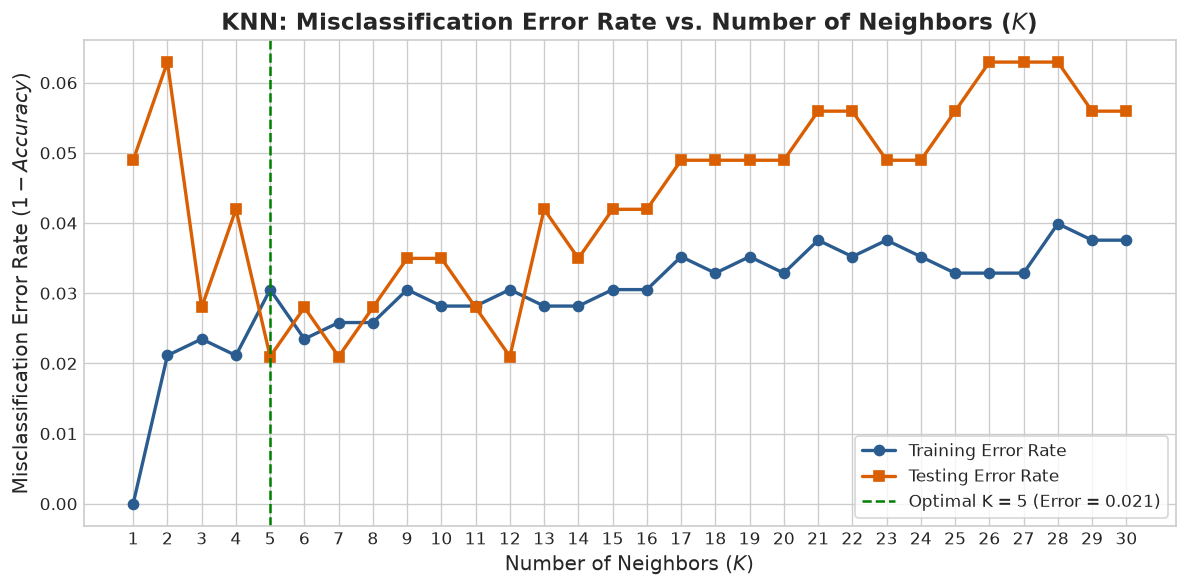
\includegraphics[width=0.75\textwidth]{figures/knn_error_vs_k.png}
    \caption{KNN Error Rate Curve across $K \in [1, 30]$ indicating minimal generalization error at $K=5$.}
    \label{fig:knn_k_curve}
\end{figure}

\begin{lstlisting}[style=output]
Optimal KNN Neighbor Count: K = 5 with Test Error: 0.0210 (Accuracy: 0.9790)
\end{lstlisting}

\newpage
\section{Comparative Evaluation and Synthesis}

\subsection{Consolidated Performance Metrics}
The optimal Decision Tree model ($\text{depth}=3$) and optimal KNN model ($K=5$) are synthesized in Table~\ref{tab:comparison}.

\begin{lstlisting}[style=code]
# Refit best models
best_dt = DecisionTreeClassifier(criterion='entropy', max_depth=best_depth, random_state=42).fit(X_train, y_train)
best_knn = KNeighborsClassifier(n_neighbors=best_k, metric='minkowski', p=2).fit(X_train_scaled, y_train)

y_pred_best_dt = best_dt.predict(X_test)
y_pred_best_knn = best_knn.predict(X_test_scaled)

comparison_df = pd.DataFrame({
    'Metric': [
        'Accuracy',
        'Misclassification Error',
        'Precision (Benign)',
        'Recall (Benign)',
        'F1-Score (Benign)'
    ],
    f'Decision Tree (depth={best_depth})': [
        f"{accuracy_score(y_test, y_pred_best_dt):.4f}",
        f"{zero_one_loss(y_test, y_pred_best_dt):.4f}",
        f"{precision_score(y_test, y_pred_best_dt):.4f}",
        f"{recall_score(y_test, y_pred_best_dt):.4f}",
        f"{f1_score(y_test, y_pred_best_dt):.4f}"
    ],
    f'KNN (K={best_k})': [
        f"{accuracy_score(y_test, y_pred_best_knn):.4f}",
        f"{zero_one_loss(y_test, y_pred_best_knn):.4f}",
        f"{precision_score(y_test, y_pred_best_knn):.4f}",
        f"{recall_score(y_test, y_pred_best_knn):.4f}",
        f"{f1_score(y_test, y_pred_best_knn):.4f}"
    ]
})

from IPython.display import display
print("=== Summary Comparison Table ===")
print(comparison_df.to_string(index=False))
display(comparison_df.style.set_caption("Comparative Performance of Decision Tree vs. KNN").hide(axis='index'))
\end{lstlisting}

\begin{lstlisting}[style=output]
=== Summary Comparison Table ===
                 Metric Decision Tree (depth=3) KNN (K=5)
               Accuracy                  0.9510    0.9790
Misclassification Error                  0.0490    0.0210
     Precision (Benign)                  0.9462    0.9677
        Recall (Benign)                  0.9778    1.0000
      F1-Score (Benign)                  0.9617    0.9836
\end{lstlisting}

\begin{table}[H]
\centering
\caption{Consolidated Performance Metrics for Decision Tree vs. KNN}
\label{tab:comparison}
\vspace{0.2cm}
\begin{tabular}{lcc}
\toprule
\textbf{Metric} & \textbf{Decision Tree (depth=3)} & \textbf{KNN ($K=5$)} \\
\midrule
Accuracy                 & 0.9510 (95.10\%) & \textbf{0.9790 (97.90\%)} \\
Misclassification Error  & 0.0490 (4.90\%)  & \textbf{0.0210 (2.10\%)}  \\
Precision (Benign)       & 0.9462           & \textbf{0.9677}           \\
Recall (Benign)          & 0.9778           & \textbf{1.0000}           \\
F1-Score (Benign)        & 0.9617           & \textbf{0.9836}           \\
\bottomrule
\end{tabular}
\end{table}

\subsection{Architectural Trade-Off Analysis}
Table~\ref{tab:tradeoffs} presents a comparative analysis of the fundamental computational and theoretical differences between the two models.

\begin{table}[H]
\centering
\caption{Algorithmic and Theoretical Trade-offs: Decision Tree vs. KNN}
\label{tab:tradeoffs}
\vspace{0.2cm}
\begin{tabular}{p{4.2cm}p{5.5cm}p{5.5cm}}
\toprule
\textbf{Property} & \textbf{Decision Tree} & \textbf{K-Nearest Neighbors (KNN)} \\
\midrule
\textbf{Learning Paradigm} & Eager learning; constructs hierarchical rules during training. & Lazy learning; defers computation until test query. \\
\addlinespace
\textbf{Feature Scale Sensitivity} & Completely invariant to monotonic feature scaling. & Highly sensitive; unscaled features distort distances. \\
\addlinespace
\textbf{Interpretability} & White-box logic; inspectable conditional branch rules. & Local neighborhood lookup; opaque global decision logic. \\
\addlinespace
\textbf{Prediction Latency} & $\mathcal{O}(\text{depth})$; logarithmic and extremely fast. & $\mathcal{O}(N \cdot d)$; computationally demanding on large $N$. \\
\addlinespace
\textbf{Decision Boundaries} & Orthogonal, axis-aligned hyperplanes. & Smooth, flexible, piecewise-linear local contours. \\
\bottomrule
\end{tabular}
\end{table}

\section{Conclusion}
In this laboratory assignment, both Decision Tree and K-Nearest Neighbors classifiers were implemented, tuned, and evaluated on the Breast Cancer Wisconsin dataset. Standard scaling was demonstrated as an imperative prerequisite for KNN, while the Decision Tree exhibited scale invariance. While KNN achieved superior test accuracy ($97.90\%$ vs $95.10\%$) and perfect recall on the benign class, the Decision Tree provided explicit interpretable rules with logarithmic inference latency. Both models exhibited predictable bias-variance trade-offs governed by tree depth and neighbor cardinality.

\end{document}
